\documentclass[11pt]{article}
\usepackage{amsmath,amsfonts}
\usepackage[numbers,sort&compress]{natbib}
\usepackage{times}
\usepackage[left=2.54cm,top=2.54cm,right=2.54cm,bottom=2.54cm,bindingoffset=0.0cm]{geometry}
\usepackage{setspace}
\usepackage{enumerate}
\usepackage{enumitem}
\usepackage{wrapfig}
\setcounter{secnumdepth}{0}
\usepackage{fullpage}
\usepackage{titlesec}
\titleformat{\section}{\large\bfseries}{\thesection}{1em}{}
\titleformat{\subsection}{\bfseries}{\thesubsection}{1em}{}
\usepackage{parskip} % skip paragraph indentations
\usepackage{lipsum}
\usepackage{hyperref}
\usepackage{graphicx}
\usepackage{amssymb}
\usepackage[x11names]{xcolor}
\usepackage{hyperref}
\usepackage{enumitem}
\usepackage{booktabs}
\usepackage{amsmath}
\usepackage{amssymb}
\usepackage{mathrsfs}
\usepackage{caption} \captionsetup[table]{singlelinecheck=false} %makes table captions left-justified
\usepackage{framed} % to add frames around comments
%\hypersetup{backref,colorlinks=false,
%    urlbordercolor=LightSkyBlue4,          % color of internal links
%    citebordercolor=SpringGreen4,        % color of links to bibliography
%    filebordercolor=magenta,      % color of file links
%    linkbordercolor=Red3, pdfborderstyle={/S/U/W 1.5}}
\newcommand{\Prob}[1]{\Pr{\left( #1 \right)}}
\newcommand{\q}[1]{``#1''} % easier way to get double quotes
\newcommand{\argmin}{\text{argmin}}
\usepackage{authblk} % for title page
\renewcommand\Affilfont{\fontsize{10}{10.8}\itshape}
\renewcommand\familydefault{\sfdefault} 
\usepackage{datetime2}
%\renewcommand{\dateseparator}{-}
\usepackage{atbegshi}% http://ctan.org/pkg/atbegshi -- removes blank page at start of doc
\AtBeginDocument{\AtBeginShipoutNext{\AtBeginShipoutDiscard}}
\setcounter{page}{0}
\begin{document}
\noindent
\title{Large group and moderate cognitive abilities favor the evolution of badges of status over individual recognition} 
%The evolution of rank signaling?

\author[1]{Eleanor R. Brush}
\affil[1]{Department of Biology, University of Maryland, 4094 Campus Dr., College Park, MD 20742; email: eleanor.brush@gmail.com}
\author[2,3]{Elizabeth A. Hobson}
\affil[2]{Santa Fe Institute, 1399 Hyde Park Road, Santa Fe, NM 87501 USA}
\affil[3]{Center for Biosocial Complex Systems, Arizona State University; email: ehobson@santafe.edu}
%\date{} 
\maketitle

Target journal: Behavioral Ecology 
%instructions: http://www.oxfordjournals.org/our_journals/beheco/for_authors/general.html
% also: http://www.oxfordjournals.org/our_journals/beheco/for_authors/submission_online.html

Target submission date: by end of November!!
%%%%%%%%%%%%%%%%%%%%%%%
\linenumbers
%%%%%%%%%%%%%%%%%%%%%%%

\section*{Abstract}

\framebox(500,100){to be added..........................................}

\textit{Keywords: badge, cognition, evolution, learning, recognition, signal, social groups,  [.....]}
\newline

%%%%%%%%%%%%%%%%%%%%%%%
\section*{Introduction} 
%%%%%%%%%%%%%%%%%%%%%%%


Animals in social groups benefit from having accurate information about their group mates. For example, knowing about the dominance \cite{Hobson:2015kx,Hobson:2015uq,Flack:2006fk,Brush:2013fk,Flack:2006uq,Cowlishaw:1990vn,Waal:1986ys}, resource holding potential \cite{Arnott:2009zr,Lemel:1993ve,Dick:1990cr}, likelihood of investing in parental care \cite{Olsen:2010uq,Qvarnstrom:1997fk}, or health \cite{Folstad:1992kx,Loyau:2005nx} of other animals can help an animal decide with whom to fight, mate, or interact. In order to learn about one's group mates, an animal must be able to identify them. There are many solutions to this problem. Some animals can recognize other members of their groups as individuals. Other animal coarsely categorize conspecifics based on traits they exhibit. When such a trait is correlated with another property of interest, for example dominance or health, it becomes a badge of status (xxxKrebsDawkins1984), which allows animals to make inferences about each others' quality as mates or opponents or allies XX. Much is known about what circumstances might promote the evolution of one or the other type of learning XX, but there are few studies that compare the two systems directly \cite{sheehan2016evotradeoff}. In this paper, we develop and analyze a simple model of an animal social group, in which animals learn by interacting with each other and by observing these interactions, in order to learn how group size and cognitive abilities affect the effectiveness of using both types of learning and to determine the circumstances under which one or the other is preferable. 

% summary of previous research on badges
There are many species in which animals have been shown to use badges of status to make inferences about each other. One well known-example is the house sparrow (XX): the size of a male sparrow's black bib is correlated with its physical condition and other sparrows seem to use this information to decide how to interact with a given male XX. Another well-studied example is the paper wasp (XX): the extent of black and the number of black patches on a wasp's face are positively correlated with its dominance, suggesting that wasps use that trait when deciding with whom to fight and how aggressively \cite{Tibbetts:2004kx}XX. Other examples include the size of the rusty cap in swamp sparrows, which is correlated with parental investment\cite{Olsen:2010uq}; the bib in great tits, which is used by other males to estimate the fighting ability of a previously unknown opponent \cite{Lemel:1993ve}; plumage brightness in house finches, which is correlated with body condition and survival \cite{McGraw:2000qf}; the number of spots in a peacock's tail, which indicates its health \cite{Loyau:2005nx}; the white patch on a collared flycatcher's forehead, which predicts its ability to attain a territory \cite{Part:1997ys}. OR include both melanin and carotenoid pigmentation in several species of birds \cite{Olsen:2010uq,Lemel:1993ve,McGraw:2000qf,Young:2015dq,Jawor:2003bh}. 
% UV signals: Blue Tits in Remy et al 2010 (http://link.springer.com/article/10.1007/s00265-010-0995-z)


% in Remy et al 2010 (http://link.springer.com/article/10.1007/s00265-010-0995-z)  "...a major assumption of the badge of status hypothesis: namely, badges of status are used between unfamiliar individuals to signal fighting abilities and aggressiveness at a distance (Maynard Smith and Harper 2003, Animal Signals )".

Previous research has been shown that XX factors promote the evolution of a badge that is correlated with quality. When a group starts to use a badge as a proxy for quality, an incentive appears for low-quality animals to ``cheat" and produce a badge that indicates they are higher quality than they actually are. Many cheaters in the system could decrease the informativeness of a signal. However, an ``honest" badge can evolve and persist if it requires individuals to pay a cost to produce, maintain, or display it. For example, some badges are energetically costly to produce, ie xxxx, while other badges may be costly to display if there is a mismatch between the badge and the individual's quality, for example when other individuals punish cheaters ~\cite{Smith2003AnimalSignals}\textit{[XXXXXadd more refs]}.  \textit{[However, even cost-free signals can maintain their honesty \cite{Dawkins:1991ly}XX.]} In order for animals to use badges of status to learn about their group mates, the badge must be informative to some extent \emph{and} the animals must pay attention to and make inferences based on the badge. While many studies have addressed the evolution and maintenance of a highly informative badge, fewer have addressed the evolution of the required type of learning (although see XX).  We therefore focus on the factors that might lead to the evolution of a learning system that relies on badges, rather than the evolution of the badges themselves.
%punishment can also maintain honesty (reviewed in Maynard-Smith and Harper 2003, Animal Signals)
>>>>>>> master

% summary of previous research on individual recognition
There are also many species that can individually recognize their group mates (reviewed in~\cite{Tibbetts2007IndividualDifferent,Wiley2013SpecificityBehaviour}). However, this recognition is likely cognitively constrained; as groups become larger and larger, it becomes more difficult to effectively and accurately learn about and remember assessments for all of one's group mates. Learning about relative quality rankings or relationships between individuals is combinatorially explosive~\cite{Seyfarth2015SocialCognition}. Even humans are thought to be limited in terms of individual recognition, where previous work has hypothesized that humans can only remember the faces of about 150 people XX. These cognitive constraints may have been important in early human evolution, especially in the context of cooperation, and may in turn have imposed social constraints, limiting early human group sizes to no more than about 150 people XX Dunbar.

%``Individual recognition" is not a prerequisite for dominance hierarchies but dominance hierarchies may be a driving force of the evolution of ``individual rcognition." \cite{Barnard:1979fk}

While badges of status and individual recognition are usually presented as fundamentally different solutions to the same biological problem, individual recognition is in some ways just an extreme version of learning about others' badges \cite{Barnard:1979fk}. Animals that make inferences about their peers based on the badges they display are limited by their perceptive and cognitive abilities: if two animals have badges that are close enough in size that others cannot tell the difference between them, their peers will judge that they have the same size badge and therefore the same ``quality." As perceptive abilities improve, an animal will be able to make finer distinctions about its peers, to the point that it may be able to recognize each of them individually. (We use vision here for the sake of clarity, but the same holds true for other senses as well.) Such a spectrum from coarse-grained to fine-grained perceptive abilities can be seen in the group of paper wasp species. In some species, wasps distinguish between other wasps based on the number of black patches on their face, a relatively coarse trait \cite{Tibbetts:2004kx}XX, whereas in some species wasps can recognize other individuals based on their unique facial patterns XX. In addition to this evidence that there is variation in animals' abilities to perceive differences, there is also evidence in some species that the animals are aware of the degree of similarity between badges \cite{Molelr:1987vn}. The correlation between the badge and another trait has received a lot of attention in previous studies of the evolution of badges of status. However, the specificity with which the badge can be perceived has not been. As we show below, it is a crucial factor in determining how effectively an animal can learn from its group mates' badges. Because the two systems are usually thought of as totally separate, they are usually studied separately \cite{sheehan2016evotradeoff}. In this paper, we explicitly compare the performance of animals using types of learning that fall across this spectrum.

Regardless of whether animals pay attention to a badge of status or focus on individual identity, they have several potential sources of information. They can learn through direct interactions. For example, when two bighorn sheep fight, they both gain information about the other's strength XX. They can also learn through observational learning. By observing the result of interactions between other pairs of animals, one can gain information about their relative abilities or sometimes even their absolute abilities. Observational learning is known to be an important avenue of learning in many species XX and is thought to be a valuable way of gathering information XX. However, the degree to which it helps an animal learn depends on the information it already has and the advantage of using observational learning may differ depending on what kind of learning an animal engages in.

Many factors influence how accurately animals can learn about their group mates. Based on  thought experiments, Sheehan and Bergman~\cite{sheehan2016evotradeoff} predicted that group size, the stability of the social group, and the stability of the badge over time should all affect how well animals using both of the two systems can learn about their peers. In this paper, we focus on modeling a subset of these ideas. Our goals are (1) to better understand how group size, memory, and perceptive ability how well animals can learn the quality of their group mates, (2) to better understand how observational learning affects how well can animals can learn, and (3) to determine the conditions under which the evolution of a badge signal or individual recognition would be favored. To address these questions, we develop a model, in which quality assessment occurs by one of two methods: (1) a badge signal system, where animals assess quality of others by grouping individuals into quality categories based on the intensity of badge signals and (2) an individual recognition system, where animals use individual recognition of their peers to assess quality to specific individuals.  


%%%%%%%%%%%%%%%%%%%%%%%
\section*{Model} 
%%%%%%%%%%%%%%%%%%%%%%%

% add 'biological basis' for some of assumptions in model
Each animal in the social group has an inherent quality value. This can be thought of, for example, as fighting ability XX, resource holding potential XX, body size, body condition, or any other property about which it would be beneficial to have information. In our basic model, an animal learns about another's quality value by interacting with it directly. We also extend our model to cases where animals can learn through observing the interactions between other pairs in addition to direct interactions. We consider two different methods of learning: individual recognition and badges. An animal using individual recognition can identify each of its group mates as a particular individual. An animal using the badge system only recognizes animals based on the signals they display in a categorical fashion. Our model assumes that it is costly to the animals in the group to learn about each other inaccurately. Since animals can use information about their group mates to decide how to interact with them in the future, having the wrong information can lead to an inappropriate choice. We also assume that it is also costly to learn slowly. The time spent interacting and learning about one's group mates could be spent in other ways. Additionally, if the interaction is actually a fight between animals, having more interactions than necessary can lead to injury and perhaps even death. Finally, we also assume that having improved memory and perceptive ability is costly because of the associated energetic costs of larger brain or because improving these properties involves a trade-off that negatively affects other traits. We combine the costs associated with inaccurate learning, the time required to learn, and cognitive abilities to assess the performance of animals using each of the two learning systems. 

\subsection{Interactions and learning }
We assign each animal a quality value, $q_i$, and a signal, $s_i$, which is always perceptible to conspecifics. We define the parameter $\rho$ as the correlation between the signals, $\{s_i\}$, and the quality values, $\{q_i\}$. In a group with $N$ animals, we draw quality values $\{q_1,\dots,q_N\}$ from a normal distribution with mean $0$ and standard deviation $\sigma_\text{q}$. We then generate $N$ signal values such that $\min_i{s_i}\approx -1$, $\max_i{s_i}\approx 1$, and the correlation between $\{q_i\}$ and $\{s_i\}$ is precisely $\rho$ (see Table~\ref{tab:vars} for a description of the variables used in the text). The question of how a signal comes to be correlated with quality is an interesting one. Some of the circumstances that can allow for this to happen include XX In the future, we plan to include an evolutionary timescale in our model and to consider the evolution of the signal, but for the moment, we assume the signal-quality correlation is fixed at a given level.
%added a little about how we don't consider/allow for cheating
We do not consider or allow for cheating in this model (i.e. lower-quality individuals cannot display a higher than expected signal intensity, all individuals display signals that are linked to their underlying quality in the same way).
  
Each animal assesses the quality of each other animal: $a_{ij}(t)$ is the opinion of animal $i$ about animal $j$ at time $t$.  At first, the group consists entirely of naive animals: at $t=0$, no animal has an opinion of any other. Every animal has a memory window of length $w$. At each point in time, first, if animal $k$ has not updated its opinion of animal $\ell$ within the last $w$ timesteps, it forgets its opinion of $\ell$. Next, two animals, $i$ and $j$, are chosen randomly to interact. If $i$ already has an opinion of $j$, its updated opinion is 
\begin{equation*}
a_{ij}(t)=(1-\ell_\text{i})a_{ij}(t-1)+\ell_\text{i} q_j+\xi,
\end{equation*}
where $\ell_\text{i}$ is a parameter describing how much $i$ changes its opinion based on the interaction and $\xi$ is drawn from a normal distribution with mean $0$ and standard deviation $\sigma_\text{i}$. If $i$ and $j$ have not previously interacted or $i$ has forgotten its opinion of $j$, then after interacting 
\begin{equation*}
a_{ij}(t+1)=(1-r)b_{i}(t)+rq_j+\xi,
\end{equation*}
where $b_i(t)$ is a baseline opinion of any animal it encounters. Specifically, $b_i(t)$ is drawn from a normal distribution with mean $0$ (the expected quality value of any animal) and standard deviation $\sigma_\text{b}$. The other animals in the group observe the interaction with probability $p_\text{o}$. If animal $k$ observes the interaction, it uses the same rules to update its opinion of both $i$ and $j$, with parameters $\ell_\text{o}$ and $\sigma_\text{o}$. We use $\ell_\text{o}\leq\ell_\text{i}$ and $\sigma_\text{o}\geq\sigma_\text{i}$ so that observational learning is noisier. This completes the description of how learning occurs for animals using individual recognition. 

\subsection{Badge system }
An animal that uses the pure badge system to learn cannot perceive the difference between animals with similar signals and is forced to make a noisy estimate of the quality values of all such animals. Specifically, an animal divides the rest of its group into categories before any interactions take place. It does so by picking another animal, $j$, at random. All animals whose signals are within $\delta/2$ of $s_j$ are put in the same category. Then the focal animal picks an uncategorized animal at random, $k$, forming a second category of all uncategorized animals whose signals are within $\delta/2$ of $s_k$. The process continues until every animal in the group has been assigned a category. Category width $\delta$ depends on the animals' perceptive abilities. For example, if $\delta$ is large, an animal might only be able to identify animals with small, medium, and large signals, whereas if $\delta=0$ an animal can identify every individual in its group and using the badge is no different than using individual recognition. Different animals will categorize the group differently and may perceive different numbers of categories. Figure \ref{cats_ex} shows one example of this process. 
%Each individual $i$ will identify a category $c$ by the median of the signal being displayed by individuals in that category, $\bar{s}_{ic}$. 
The average number of categories  animals perceive decreases with group size and category width, $\delta$ (Figure \ref{num_cat}). When an animal using the badge system updates its opinion of another animal based on direct interaction or on observation, it simultaneously updates its opinions of all the other animals in the same category. If an animal observes an interaction between two animals in the same category, it does not updates its opinion of that category.
%Add something about how badge learners with delta=0 are equivalent to individual recognition except in how they make errors. See Appendix.

%A categorical learner re-categorizes the rest of the group at each time step. Specifically, animal $i$ puts animal $j$ in category $k$ with probability 
%\begin{equation*}
%\frac{\exp(-r_\text{cat}|s_j-\bar{s}_{ik}|)}{\sum_\ell\exp(-r_\text{cat}|s_j-\bar{s}_{il}|)},
%\end{equation*}
%where $r_\text{cat}$ describes the reliability of the categories over time: if $r_\text{cat}=\infty$, $i$ categorizes the group the same way at every time step and as $r_\text{cat}$ the probability of re-categorizing animals increases. If $i$ remembers its opinion of category $k$, it assigns that opinion to all individuals it now perceives as being in category $k$. 
%The animal with higher quality is more likely to win. Specifically, the probability of $i$ winning in a fight against $j$ is 
%\begin{equation*}
%\frac{\exp\big(b(q_i-q_j)\big)}{\exp\big(b(q_i-q_j)\big)+1},
%\end{equation*}
%where $b$ represents the bias in the fight: if $b=0$, then both animals are equally likely to win, regardless of their qualities, and if $b$ is large, the stronger animals wins with near certainty. 
%An individual learner correctly identifies its opponent with probability $r_\text{ind}$. With probability $1-r_\text{ind}$ it misidentifies its opponent as another randomly chosen member of the group.  A categorical learner perceives the category of its opponent with the probabilities just described. Each animal in the fight updates its opinion of the individual or category it perceives in its opponent. If $a_{ij}(t-1)$ is $i$'s opinion of $j$ at time $t-1$, after fighting, 
 
\subsection{Measures of performance }
The animals interact and learn about each other for $T$ timesteps. To measure each animal's learning ability, we average the errors it makes in its opinions about the rest of the group: 
\begin{equation*}
\epsilon_i(T) = \frac{1}{|\mathscr{O}_i(T)|}\sum_{j\in \mathscr{O}_i(T)}|a_{ij}(T)-q_j|,
\end{equation*}
where $\mathscr{O}_i(T)$ is the set of animals about whom $i$ has an opinion at time $T$.  
We also calculate the average time it takes for an animal's error about each other animal to drop below a threshold:
\begin{equation*}
\tau_{i} = \frac{1}{|\mathscr{O}_i|} \sum_{j\in\mathscr{O}_i} \min_{t=1,\dots,T}\{t: \epsilon_{ij}(t)\leq 0.2 \}.
\end{equation*}
(If $\epsilon_{ij}$ is always greater than the threshold, then $i$'s learning time about $j$ is taken to be $T$.) Figure \ref{learnT.ex} shows one example of this calculation. We model $25$ groups of animals using each of the two learning systems and calculate the average error $\bar{\epsilon}$ and average learning time $\bar{\tau}$ of all animals in all groups. In Figure \ref{learning_curves} we show how the average error of animals using each of the two systems changes over time.

Learning errors and learning time can both be costly. Individuals can gain long-term benefits from assessing each others' quality. 
%In the context of conflicts when individuals differ in fighting ability, resource-holding potential, or dominance rank, individuals can benefit [through decreased chances of injury, increased chances of outcome success, etc.] if they are able to identify and order individuals by quality.  
Improving  perceptive ability (by decreasing $\delta$) and improving memory (by increasing $w$) can also be costly XX. %need some citations / ties to biology here? Maybe cost of cognition involved in increasing memory?

We describe the cost of the category width with the function
\begin{equation*}
c_\delta = \left(\frac{2-\delta}{2}\right)^\alpha
\end{equation*}
and that of memory with the function
\begin{equation*}
c_w = \left(\frac{w}{2000}\right)^\alpha,
\end{equation*}
where $\alpha$ is a parameter determining the concavity of the cost function. The animals pay no costs for having no cognitive ability ($\delta=2$ and $w=0$), and $1$ unit of cost for optimal cognitive ability ($\delta=0$ and $w=2000$, the highest $w$ we consider). (Figure \ref{cost_fx} shows these cost functions.)
We then combine the four sources of cost---error, time, memory window, and category width---into the total cost 
\begin{equation*}
C = 2\bar{\epsilon}+10^{-4}\bar{\tau}+c_w+c_\delta,
\end{equation*}
where the terms in front of $\bar{\epsilon}$ and $\bar{\tau}$ ensure that the four factors, $\bar{\epsilon}$, $\bar{\tau}$, $c_w$ and $c_\delta$, are on the same scale. 

%
\begin {table}[ht]
\caption {Description of variables} \label{tab:vars} 
\begin{tabular}{cl}
\toprule
 Variables & Description of variables \\
\midrule 
$C$ & total cost of learning \\ 
$\delta$ & category width \\
$\epsilon_i$ & average error of animal $i$ about all other animals \\
$\bar{\epsilon}$ & average error of all animals in all groups \\
$\ell_\text{i}$ & learning rate in direct interaction \\
$\ell_\text{o}$ & learning rate in indirect observation \\
$N$ & number of animals in group \\ 
$p_\text{o}$ & probability of observing interactions between other pairs \\
 $q_i$ & quality of animal i \\ 
 $\rho$ & correlation between quality and signal \\
$s_i$ & signal of quality / badge of status of animal $i$ \\ 
$\sigma_\text{b}$ & standard deviation of baseline opinion \\
$\sigma_\text{i}$ & standard deviation of noise in opinion updating during interaction \\
$\sigma_\text{o}$ & standard deviation of noise in opinion updating during observation \\
$\sigma_\text{q}$ & standard deviation of quality values \\
$T$ & total number of fights \\
$\tau_i$ & average learning time of animal $i$ \\
$\bar{\tau}$ & average learning time of all animals in all groups \\ 
$w$ & memory window \\
\bottomrule
\end{tabular}
\end {table}
%

%%%%%%%%%%%%%%%%%%%%
\section*{Results}
%%%%%%%%%%%%%%%%%%%%

%
\subsection*{The effects of group size and cognitive abilities on learning }
We first analyze the model without any observational learning ($p_\text{o}=0$). We compared three parameter combinations to visualize how average error decreases over time (Figure~\ref{learning_curves}). Average errors in quality assessment generally decreased over time until errors stabilized and were no longer affected by the number of interactions. Stabilization of errors is indicative that maximum learning has been reached. In most cases, this maximum learning point was reached much more quickly in the categorical badge system than in the individual recognition system [\textit{hard to tell exactly with panel C, does indiv recog stabilize before badge there?}]. Badges with lower signal to quality correlation strengths (R=0.5) resulted in the largest errors in quality assessment across all three comparisons (dotted red lines, Figure~\ref{learning_curves}). Individual recognition in small groups (N=20) resulted in the most accurate quality assessments of all comparisons, but required a large number of interactions before this accurate assessment was reached (Figure~\ref{learning_curves}A). In larger groups (N=50), many more interactions were required for the individual recognition systems to become accurate, and assessment did not reach the accuracy seen in small groups. Quality assessment under both badges and individual recognition were less accurate when group size increased, and the accuracy of individual recognition was more affected than in the badge system (Figure~\ref{learning_curves}B). Error rates were even higher when we compared larger groups with a long memory span (Figure~\ref{learning_curves}B) to larger groups with a smaller memory span (Figure~\ref{learning_curves}C). In this case, when we decreased the memory span of individuals, the error in quality assessment in individual recognition increased, and average errors were higher when memory was shorter, although individual recognition still outperformed the badge with lower signal to quality correlation. 

\begin{figure}

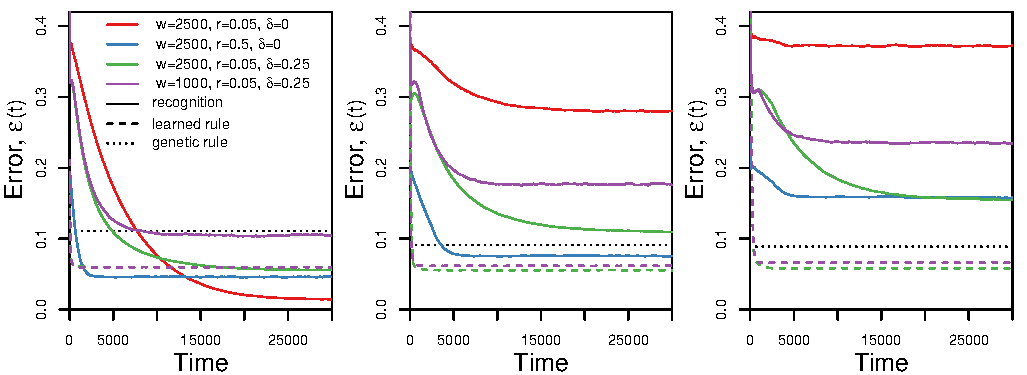
\includegraphics[width=.95\textwidth]{figures/learning_curves.pdf}
\caption{\label{learning_curves} \sffamily\small\textbf{Examples of how average error decreases over time.}
In each panel, we show time in number of interactions on the x-axis and average error, $\bar{\epsilon}$, on the y-axis. The line shows the average error across all animals in all groups and the shaded area shows this average $\pm 0.5$ the standard deviation of error across all animals in all groups. In each panel, blue lines show animals using individual recognition and red lines show animals using the badge system. The solid lines correspond to groups where signal-quality correlation $\rho=0.9$ and the dotted lines correspond to groups where signal-quality correlation $\rho=0.5$. As groups size increases, from A to B, the error of animals using both systems increases, but it affects the error of animals using individual recognition more. As memory window decreases, from B to C, the error of animals using the badge system is not strongly affected, whereas the error of animals using individual recognition becomes higher. Parameters: in all panels $\delta = 0.5$, $\ell_\text{i}=0.2$, $p_\text{o}=0$, $\sigma_\text{b}=0.2$, $\sigma_\text{i}=0.01$, $\sigma_\text{q}=0.5$, $T=10000$; in A $N=20$, $w=2000$; in B $N=50$, $w=2000$; in C $N=50$, $w=500$. }
\end{figure}

\begin{figure}
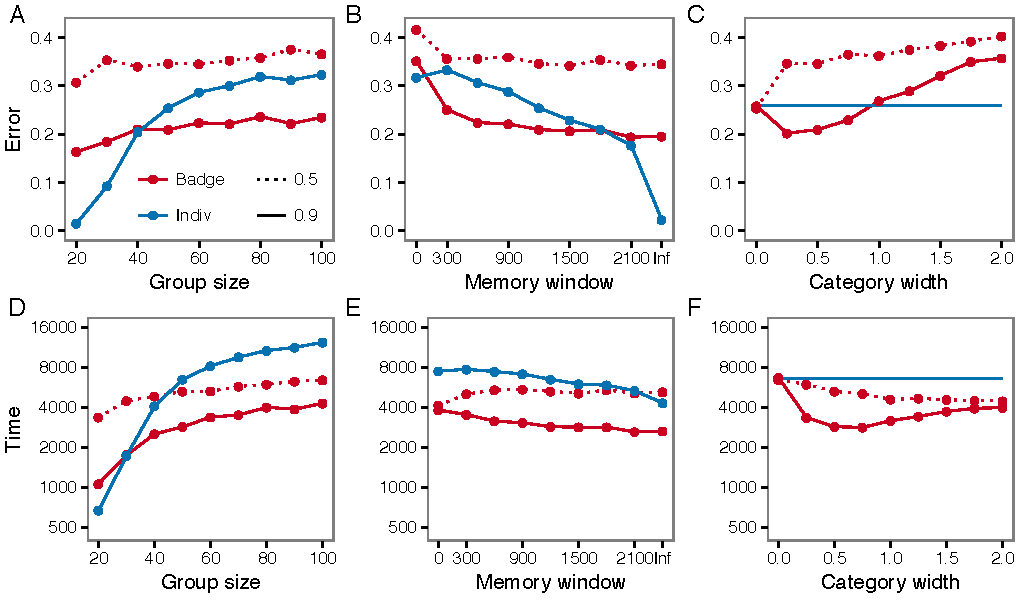
\includegraphics[width=6.85in]{figures/parameters.pdf}
\caption{\sffamily\small\textbf{Decreasing group size and increasing memory window both improve learning in the absence of observation.} Error and learning time are minimized at an intermediate category width. In the left column, we show average error $\bar{\epsilon}$ as a function of various parameters, and in the right column, we show average learning time $\bar{\tau}$ as a function of various parameters. In each panel, blue lines show animals using individual recognition and red lines show animals using the badge system. The solid red lines correspond to groups in which the signal-quality correlation $\rho=0.9$ and the dotted lines correspond to groups in which the signal-quality correlation $\rho=0.5$. Parameters: unless the parameter is being varied $\delta = 0.5$, $\ell_\text{i}=0.2$, $N=50$, $p_\text{o}=0$, $\sigma_\text{b}=0.2$, $\sigma_\text{i}=0.01$, $\sigma_\text{q}=0.5$, $T=10000$, $w=1100$.}
\label{parameters}
\end{figure}

% Fig 'parameters' description
The effects of group size $N$, memory window $w$, and signal-quality correlation $\rho$ on error and learning time are intuitive and confirm that our model is a reasonable description of a real social system. For animals using both learning systems, smaller groups and longer memory windows make it easier to learn. As group size decreases, both error and learning time decrease (Figure~\ref{learning_curves}A,B; Figure~\ref{parameters}A,B). As memory window increases, error decreases and learning time either slightly decreases or stays constant (Figure~\ref{parameters}B,C). Longer memory windows more effectively reduce error for animals using individual recognition. For animals using the badge system with moderate category widths, they encounter other animals in the same category so often that they rarely forget their opinions before the memory window has elapsed. Only when category width is very small does increasing memory window have a significant effect on error (SI?? Figure~\ref{interactions_badge}). When we compared learning for two badge signals, one with a high badge to quality correlation and one with lower badge to quality correlation, we find that badges with higher correlations with quality always outperformed badges with lower quality correlations (Figure~\ref{parameters}, solid vs dashed red lines). Animals using the badge system learn more accurately and more quickly when the the signal and quality are more strongly correlated.

%While changing any of these first three parameters (group size, memory window, and correlation)  either increased or decreased both error and learning time, changing category width led to a tradeoff between error and learning time, increasing one while decreasing the other. Increasing category width results in low learning time and high error (Figure~\ref{parameters}). When a focal animal lumps many of its peers together, it updates its opinion about each of those animals more frequently and by chance may at any given point in time have an accurate opinion about one of the animals in the category, leading to a lower average learning time. On the other hand, by lumping many animals into the same category, it loses its ability to accurately learn about their individual quality values, leading to a higher average error. 
 
When the signal is highly correlated with quality, an intermediate category width minimizes error (Figure~\ref{parameters}). This pattern can be explained as follows. Regardless of the signal-quality correlation, as category width increases, the number of animals in a given category increases (Figure \ref{num_cat}). The first consequence of this is that an animal trying to learn about a single category will encounter it more often and be less likely to forget its opinion of it before its memory window lapses, assuming its memory window is finite. This tends to decrease the error with which animals can learn about their peers. The second consequence is that each time an animal encounters a category it extrapolates the information it gathers to more animals. This tends to increase learning error. When the badge is poorly correlated with quality, this increase in error due to increased confusion is much greater than the decrease in error due to a lower chance of forgetting so that as category width increases error increases as well. However, when the badge is highly correlated with quality, the increase in error due to increased confusion is much less pronounced because animals with similar badges do actually have similar quality values. Therefore, as category width increases, at first error decreases because of the reduced probability of forgetting and later it increases because of increased confusion. Similarly, an intermediate category width minimizes learning time when the badge-quality correlation is high. When the memory window is infinite, there is no decrease in error because there is no chance of forgetting what has been learned (Figure~\ref{interactions_badge}).
%
\subsection*{The effect of observational learning}
Observational learning helps animals using both systems to learn more accurately and more quickly, but it helps animals using individual recognition much more (Figure \ref{observational}). Observational learning increases the number of animals about which a focal animal can learn at any given time. 
Observational learning increases the number of animals about which a focal animal can learn at any given time; since animals using the badge system already learn about multiple animals at once, increasing the probability of observing interactions does not have a strong effect on learning rates in badge systems.
In fact, for animals using individual recognition, the same level of error can be achieved by increasing the probability of observing ($p_\text{o}$), by increasing memory window ($w$), or by increasing both to a lesser degree. The same is true of learning time. This can be seen in the strong interaction in how error and learning time change as a function of the probability of observing ($p_\text{o}$) and memory window ($w$) (Figure~\ref{observational}).


\begin{figure}
% LIZ: I kind of like having a legend in the first panel of a plot but here it gets squished a little so I also put one in the lower left panel. I can use whichever you prefer.
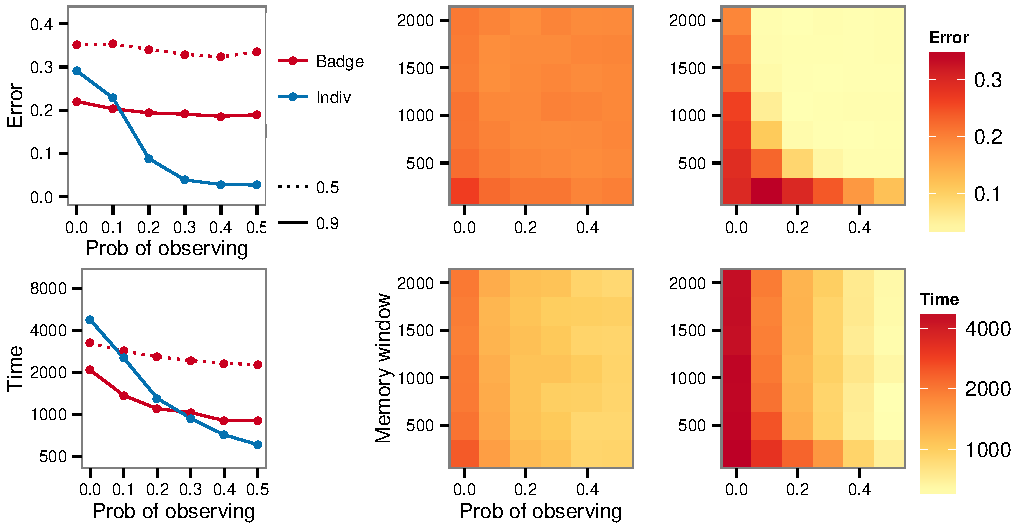
\includegraphics[width=6.85in]{figures/observational_learning.pdf}
\caption{\sffamily\small\textbf{Observational learning improves both error and learning time and does so much more for animals using individual recognition.} For animals using individual recognition, there is a strong interaction between the probability of observing and memory window. In A and D, we show average error $\bar{\epsilon}$ and average learning time $\bar{\tau}$ respectively as a function of the probability of observing, $p_\text{o}$. In each panel, blue lines show animals using individual recognition and red lines show animals using the badge system. The solid red lines correspond to groups in which the signal-quality correlation $\rho=0.9$ and the dotted lines correspond to groups in which the signal-quality correlation $\rho=0.5$. In B and C we show average error $\bar{\epsilon}$ of animals using the badge system and individual recognition respectively as a function of both the probability of observing $p_\text{o}$ on the horizontal axis and memory window $w$ on the vertical axis. In E and F we show average learning time $\bar{\tau}$ of animals using the badge system and individual recognition respectively as a function of both the probability of observing $p_\text{o}$ on the horizontal axis and memory window $w$ on the vertical axis.  Parameters: in all panels $\delta = 0.5$, $\ell_\text{i}=0.2$, $\ell_\text{o}=0.2$, $N=50$, $\sigma_\text{b}=0.2$, $\sigma_\text{i}=0.01$, $\sigma_\text{o}=0.01$, $\sigma_\text{q}=0.5$, $\rho=0.9$, $T=10000$; in A and D $w=1100$, in B and E $\rho=0.9$.}
\label{observational}
\end{figure}

%
\subsection*{Cost of learning}
%I think we should more clearly specify if this is with or without observation
% 
Since increasing group size increases both error and learning time (Figure~\ref{parameters}A,B), it also increases the overall cost of using both learning systems (Figure~\ref{costs}A). The effects of memory window ($w$) and category width ($\delta$) on overall cost depend on the cost function, specifically on the parameter $\alpha$ (Figure \ref{costs}B,C). When $\alpha<1$, the costs of memory window ($c_w$) and category width ($c_\delta$) increase most quickly at low cognitive ability; when $\alpha>1$, the costs of memory window and category width increase most quickly at high cognitive ability (Figure~\ref{cost_fx}). 

When the costs of the memory window increase quickly at low $w$ ($\alpha<1$), the rapid increase in the cost of using a longer memory window is almost exactly offset by the decrease in error and learning time, so the costs of using both systems are almost a constant function of memory window (Figure~\ref{costs}B). However, when the cost of memory window increases quickly at high $w$ ($\alpha>1$), overall costs initially decrease as $w$ increases because of the improvement in error and learning time and only eventually increase because of the cost of using a longer memory window, so an intermediate memory window is the least costly (Figure~\ref{costs}B).

Using a category width $\delta$ equal to $0$ is always costly because it leads to high error and learning time, as we saw above (Figure~\ref{parameters}E,F).  When the costs of category width increase quickly as $\delta$ decreases from $2$ ($\alpha<1$), overall costs tend to increase as $\delta$ decreases, but there is a large range of intermediate $\delta$ at which overall costs are nearly constant: in this range, the increase in cost from decreasing $\delta$ is offset by a decrease in cost from reduced error and learning time. When the costs of category width increase only at low $\delta$ ($\alpha>1$), at first decreasing $\delta$ decreases overall cost by improving error and learning time and only at low $\delta$ does overall cost increase because of the higher cost of this cognitive ability: an intermediate category width is favored (Figure \ref{costs}C).

The overall costs of using the badge system are higher than the costs of using individual recognition when group size is small and memory window is long (Figure~\ref{comparison}A,C). In these cases, animals using individual recognition are capable of learning accurately about their peers and there is no benefit from grouping animals together into categories. When the signal-quality correlation is high, individual recognition is only better for very small groups and very long memory windows (Figure~\ref{comparison}C). 

At an intermediate group size ($N=50$), animals using individual recognition perform similarly to or better than animals using the badge system when category width is small and memory window is long (Figure \ref{comparison}B,D). In these cases, animals using the badge system are paying high costs for their cognitive abilities without receiving much benefit from either improved error or improved learning time. When the signal-quality correlation is high, individual recognition is more costly except when category width is equal to $0$ and the two systems are equivalent (Figure~\ref{comparison}D). 

\begin{figure}
%I think we should more clearly specify if this is with or without observation
%and shouldn't we add a second row with observational learning included here?
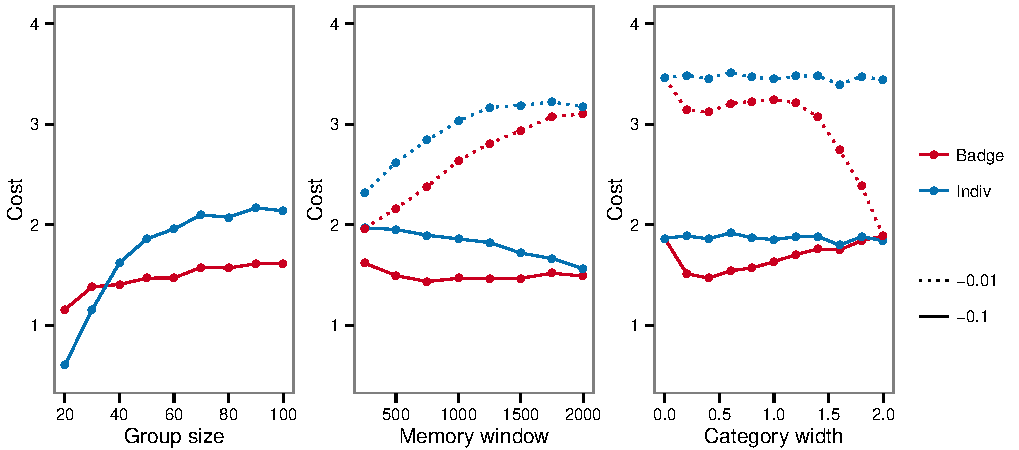
\includegraphics[width=6.85in]{figures/costs.pdf}
\caption{\sffamily\small\textbf{When individuals learn through direct experience, overall costs are lowest in small groups and with intermediate memory window and category width, when costs increases at high cognitive abilities ($\alpha>1$).} When costs increase at low cognitive abilities ($\alpha<1$), memory window $w$ does not affect overall costs and large category width $\delta$ minimizes overall costs. In A,B, and C, we show overall costs $C$ as a function of group size $N$, memory window $w$, and category width $\delta$ respectively. In each panel, blue lines show animals using individual recognition and red lines show animals using the badge system. The solid lines correspond to $\alpha=5$ and the dotted lines correspond to $\alpha=0.2$.  Parameters: unless the parameter is being varied $\delta = 0.5$, $\ell_\text{i}=0.2$, $N=50$, $p_\text{o}=0$, $\rho=0.9$, $\sigma_\text{b}=0.2$, $\sigma_\text{i}=0.01$, $\sigma_\text{q}=0.5$, $T=10000$, $w=1100$.}
\label{costs}
\end{figure}

\begin{figure}
%I think we should more clearly specify if this is with or without observation
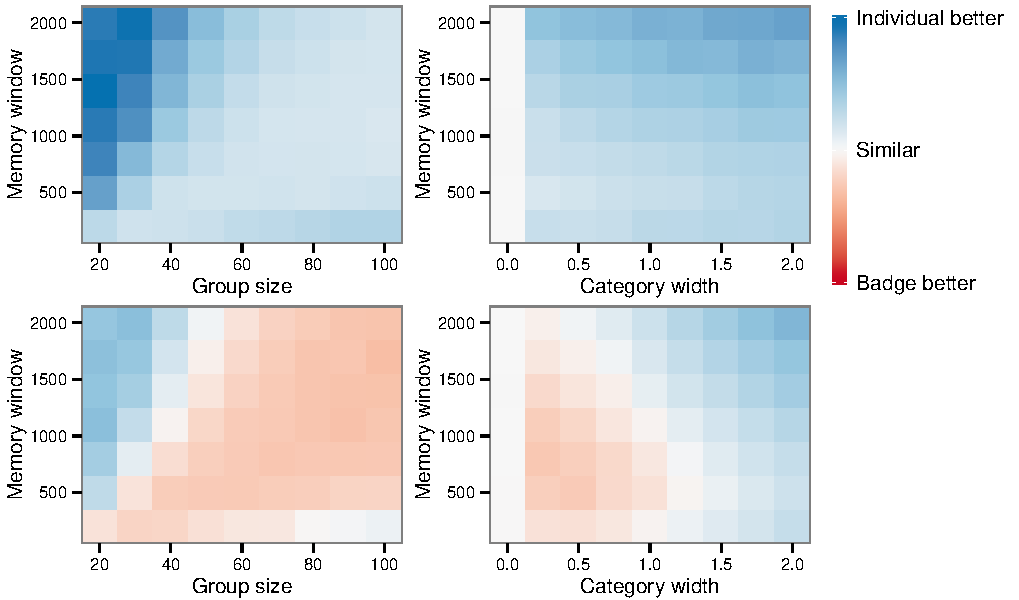
\includegraphics[width=6.85in]{figures/cost_comparisons.pdf}
\caption{\sffamily\small\textbf{The overall costs of using individual recognition are lower than the costs of using the badge system at low group size, high memory window, and low category width.} When the signal-quality correlation $\rho$ increases, animals using the badge system incur lower costs for more combinations or parameters. Here we show the difference in the overall costs ($C$) associated with individual recognition and with the badge system as a function of A,C group size $N$ and memory window $w$ and B,D category width $w$ and memory window $w$. Red indicates the badge system is less costly and blue indicates individual recognition is less costly. Parameters: in A and B $\rho=0.5$, in C and D $\rho=0.9$; unless the parameter is being varied $\delta = 0.5$, $\ell_\text{i}=0.2$, $N=50$, $p_\text{o}=0$, $\sigma_\text{b}=0.2$, $\sigma_\text{i}=0.01$, $\sigma_\text{q}=0.5$, $T=10000$, $w=1100$.}
\label{comparison}
\end{figure}

%%%%%%%%%%%%%%%%%
\section*{Discussion}
%%%%%%%%%%%%%%%%%

% Study question, restated/reframed
Accurate assessment of the quality of conspecifics is important in many contexts, but the conditions under which different assessment systems may be favored is not well understood. Here, we modeled quality assessment in social groups, with animals using either a badge signal, which allows them to group others into quality categories based on the intensity of the badge, or individual recognition, where they remember the outcomes of events involving each particular individual. Our goal was to better understand the costs and benefits of each system and the conditions under which each system might be favored. 

\subsection*{Summary of results (no costs) and implications} %temporary heading
In the absence of observational learning, smaller groups and longer memory duration make it easier to learn in both learning systems, which is consistent with general intuition. While the sign of the effect of increasing group size was the same in the two systems, the extent of the effect differed between. Assessment error and learning time were much more affected by increasing group size in the individual recognition system than the categorical badge system. We also find that agents using the badge system learn more quickly and accurately when there is a strong correlation between the signal and quality. While the correlation values we use are a bit higher than those estimated in species for which this data has been collected (XX  paper wasps \cite{Tibbetts:2004kx}, house sparrows \cite{Veiga:1993fk}, swamp sparrows \cite{Olsen:2010uq}, see Table \ref{corr_examples} for details), our model shows that even with a moderate correlation the badge system is an effective way to learn about one's group mates. 
%%%COMPARE TO \cite{sheehan2016evotradeoff} but slightly different because they assumed badge learners have an innate knowledge of what the badge means

%In the badge system, we also find that changes in the discrimination ability of agents (category width) led to a trade-off between error and learning time, with increasing category width resulting in lower average learning time but higher error. This is because when a focal animal lumps many of its peers together, it updates its opinion about each of those animals more frequently and by chance may at any given point in time have an accurate opinion about one of the animals in the category, leading to a lower average learning time. On the other hand, by lumping many animals into the same category, it loses its ability to accurately learn about their individual quality values, leading to a higher average error. 

We also find that animals using the badge system could minimize both the error with which they learned and their learning time by having a moderate ability to discriminate between different badges (i.e. by using an intermediate category width), as long as the badge was highly correlated with the underlying quality. This is somewhat counterintuitive as one might expect that it would always be advantageous to improve one's cognitive abilities. Our finding is related to the bias-variance tradeoff in statistics and machine learning: as a statistical model becomes more complex, it is more likely that its predictions will be accurate, but its predictions become more contingent on the training set and are therefore more variable XX. Similarly, as animals increase the number of categories into which they place their peers, it becomes easier for them to learn accurately about each of those categories, but they forget their assessments more quickly and therefore have more variable assessments over time. 

One explanation for why animals have imperfect cognition is that there are costs involved in improving their cognition XX \cite{Gavrilets:2006fk}. However, our results suggest that imperfect cognition itself may be adaptive. This may explain empirical examples of imperfect cognition (e.g. \cite{Kikuchi:2010ys} XX). Also \cite{Stoddard:2011zr}?
Other studies have also found that the most advanced cognitive strategies are not always optimal \cite{Brush:2016kx,Kerr:2003vn,Dunlap:2009vn,Stephens:1991fk}. Our work therefore contributes to our growing understanding of the circumstances that do or do not lead to the evolution of sophisticated cognition.

When we allow the animals in our model to learn by observing interactions between other pairs of animals, they are able to learn more quickly and accurately in both systems, but observational learning was more beneficial for animals using individual recognition. While previous work has shown the benefits of observational learning XX, our study is the first to show that this depends on how learning occurs int the first place. Our finding is somewhat surprising because one might expect that making more observations helps animals using the badge system to make up for the deficit inherent in their categorical method of learning. However, our finding agrees with / Indeed, our finding disagrees with XX Many animals that use individual recognition also use observational learning XX. Scientists have argued that this is because both individual recognition and observational learning require advanced social cognition, of which animals using a badge system are not capable XX. However, our results suggest that it may be because it is precisely in those species that observational learning is most advantageous.

\subsection*{Summary of cost results and implications} %temp heading
We find that, depending on how quickly the explicit costs of cognitive traits increase as the traits improve, the costs of using either strategy are minimized by either not investing at all in cognition or investing in a moderate cognitive trait (either memory window or perceptive ability). We find no cases where the benefits of using the most advanced cognitive trait available (either a very long memory window or category width equal to $0$) outweighed the cost of using such a trait. This finding reinforces previous studies that showed how difficult it is for advanced cognition to evolve XX \cite{Kerr:2003vn}.



\subsection*{Evolution of assessment systems} %temp heading

We find that the categorical badge system is usually less costly than individual recognition, except when group sizes are small or their cognitive abilities are sophisticated. Not surprisingly, the higher the correlation between the badge and quality, the greater the advantage of using the badge system, since the badge becomes a more informative signal of the property animals are trying to estimate. With a long memory window and a strong correlation between badge and quality, the badge system was preferable in groups with more than about 30-40 individuals; with a weaker correlation between badge and quality, groups had to be larger than about 50-60 individuals in order for the badge system to be preferable. The advantage animals using the badge system have over animals using individual recognition increases as their cognitive abilities diminish, since their performance is not strongly affected and they pay fewer costs for investing in cognition. This finding agrees with previous studies that found that individual recognition is most useful in small groups XX \cite{Veiga:1993fk}. In particular, Dunbar has argued that early human societies were limited by the number of other people a person can effectively learn about XX. While our threshold of a group size 50-60 is not identical to his threshold of a group size of 150, they are of the same order of magnitude. Our finding also agrees with previous studies of badges of quality, which have found that badges are more likely to evolve in large groups with poor cognitive ability XX. By explicitly comparing the two systems, we have generated a prediction about the types of groups and species in which we expect one or the other system to evolve. Testing this prediction is left for future work. 


% under which kinds of natural conditions should we expect to see 1 system vs another?
%``[The individual-recognition] hypothesis is especially relevant for species with moderately sized flocks, in which the probability of repeated encounters between the same individuals is great and the value of being recognized is high (Whitfield 1987). These conditions are rare among breeding house sparrows, whose colonies frequently contain several dozen pairs in a small area and many bachelors that arrive throughout the breeding season (pers. obs.) " \cite{Veiga:1993fk}. Also highlights the need to study group dynamics.


% Learning, recognition, evolution of cognitive complexity / brain size
%Previous modeling of the evolution of cognitive complexity shows that increases can occur on the scale of 10-20 generations (Gavrilets \& Vose 2006 - the dynamics of Machiavellian intelligence) <<ABSTRACT QUOTE:...our results suggest that the mechanisms underlying the ‘‘Machiavellian intelligence’’ hypothesis can indeed result in the evolution of significant cognitive abilities on the time scale of 10 to 20 thousand generations. We show that cerebral capacity evolves faster and to a larger degree than learning ability. Our model suggests that there may be a tendency toward a reduction in cognitive abilities (driven by the costs of having a large brain) as the reproductive advantage of having a large brain decreases and the exposure to memes increases in modern societies.>>
 
\subsection*{Future steps and Conclusion}
%caveat: we're not studying an ingrained badge system like in the original review paper. Our badge system is somewhere in between that and individual recognition. Exploring the full spectrum might be interesting in the future. 
%...Lots of investigation into evolution of 'honest' signaling...  [but we don't want to get bogged down here, we're assuming a purely honest system, just with variation in how well coordinated the signal is with quality]
 
By studying a rather simple model, we were able to identify the conditions under which each system is most effective and under which one or the other system should evolve. There are further steps towards improving the realism of the model that will also improve our predictions about the evolution of the two learning strategies. XX

Our study shows that is not enough to study the conditions that could allow for the evolution of a particular type of learning. By considering and comparing two solutions to the same biological problem we find that different conditions favor different solutions. %%Eleanor just wrote this and knows it needs work!  

%%%%%%%%%%%%%%%%%
\section*{Acknowledgments}
%%%%%%%%%%%%%%%%%
Part of this work was conducted while E.A.H. was a Postdoctoral Fellow at the National Institute for Mathematical and Biological Synthesis, an Institute sponsored by the NSF, the U.S. Department of Homeland Security, and the U.S. Department of Agriculture through NSF Award \#DBI-1300426, with additional support from the University of Tennessee, Knoxville.

%%%%%%%%%%%%%%%%%%%%%%%%%%%%%%%%%%%%%%%%%%
\newpage
\bibliography{BIB_badgeVSrecog,TODO_newrefs,Mendeley_Badge_vs_Recognition.bib}
\bibliographystyle{unsrt}

\clearpage{}
%\newpage{}
\renewcommand{\thesection}{}
\section{Supporting information}
\renewcommand{\thesection}{S}
\renewcommand{\thesubsection}{S\arabic{subsection}}
\renewcommand{\theequation}{S\arabic{equation}}
\renewcommand{\thetable}{S\arabic{table}}
\renewcommand{\thefigure}{S\arabic{figure}}
\setcounter{equation}{0}  
\setcounter{figure}{0}
\setcounter{table}{0}

\begin{figure}[ht]
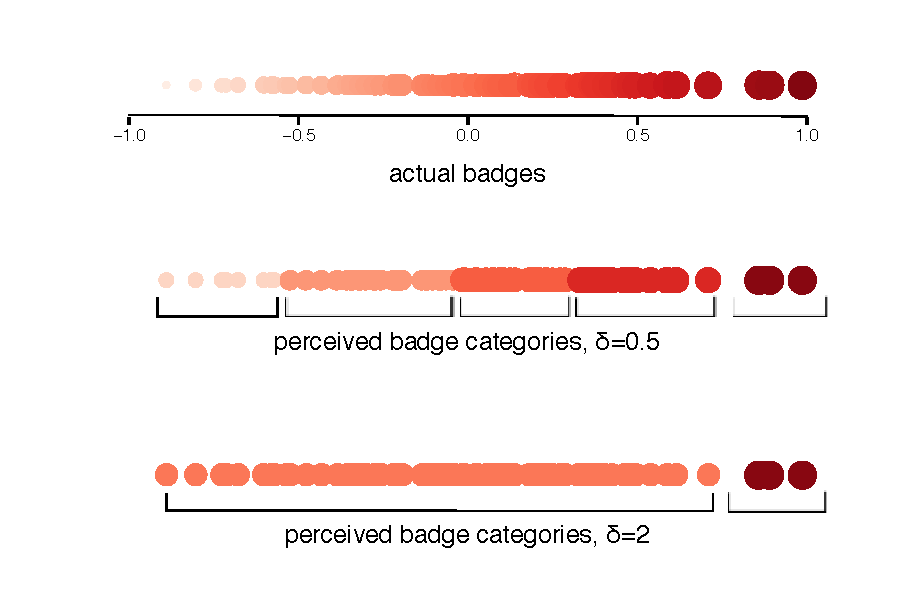
\includegraphics[width=.8\textwidth]{figures/categories.pdf}
\caption{\sffamily\small\textbf{Example of how categories are defined.}
Here we show how a group of size $N=40$ might be divided into categories with maximum width $0.5$. Each point corresponds to an animal in the group. We show the signal of each animal on the y-axis and the order of the animals from lowest to highest signal on the x-axis. The color of the point indicates the category to which it belongs and the horizontal lines show the median signal value for each category. Categories were formed by choosing an animal $i$ at random, putting all other animals whose signals were within $\delta/2$ of $i$'s signal $s_i$ into the same category, then choosing another uncategorized animal at random, and continuing until all animals were categorized.}
 \label{cats_ex}
\end{figure}

\begin{figure}[ht]
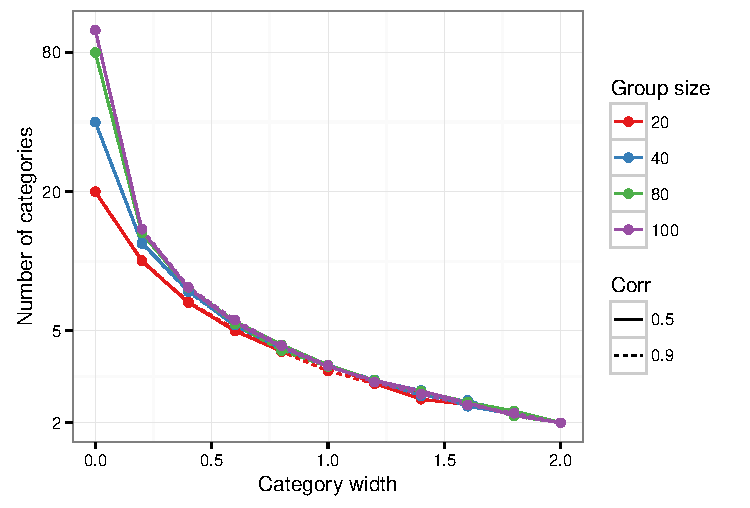
\includegraphics[width=.8\textwidth]{figures/number_of_categories.pdf}
\caption{\sffamily\small\textbf{As category width $\delta$ decreases the number of categories into which the group is divided increases.}
For a given group size $N$ and category width $\delta$ we generated a group with $N$ signal values $\{s_i\}$ and categorized the group according to the procedure in the text and Figure \ref{cats_ex} $100$ times and took the average number of categories across these $100$ groups. Here we show how the average number of categories into which a group is divided depends on group size $N$ and category width $\delta$.  Each colored line corresponds to a group size. There are overlapping solid and dotted lines in each color since the signal-quality correlation $\rho$ does not affect the number of categories formed. When $\delta=0$ there are as many categories as there are animals in the group. When $\delta=2$ there are on average $2$ categories, although it can happen that all animals are put into the same category. }
\label{num_cat}
\end{figure}

\begin{figure}[ht]
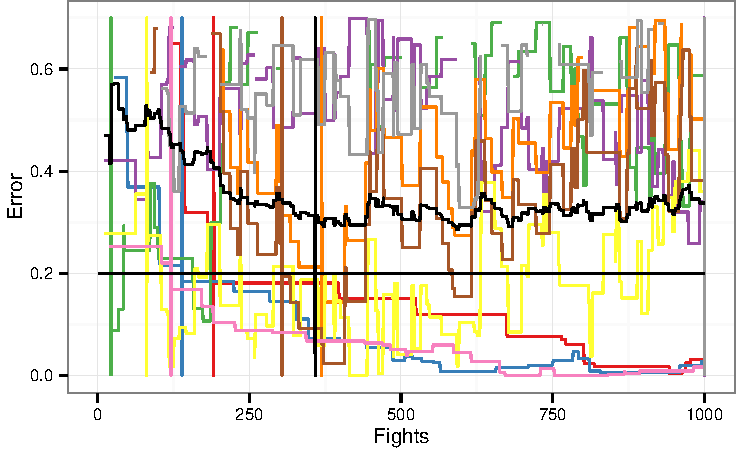
\includegraphics[width=.8\textwidth]{figures/learning_time_example.pdf}
\caption{\label{learnT.ex} \sffamily\small\textbf{Example of how to calculate learning time.} Learning time $\tau_i$ can be less than $T$, even if average error at time $T$ is above the threshold $0.2$. Each colored line shows how one the error in one animal's opinion of its five group mates changes over time. The black line is its average error about the other animals, $\epsilon_i(t)$. The horizontal black line is the error threshold, $0.2$. Each vertical colored line is the first time when corresponding line drops below the threshold. The vertical black line is the average of these learning times, $\tau_i$.}
\end{figure}

\begin{figure}[ht]
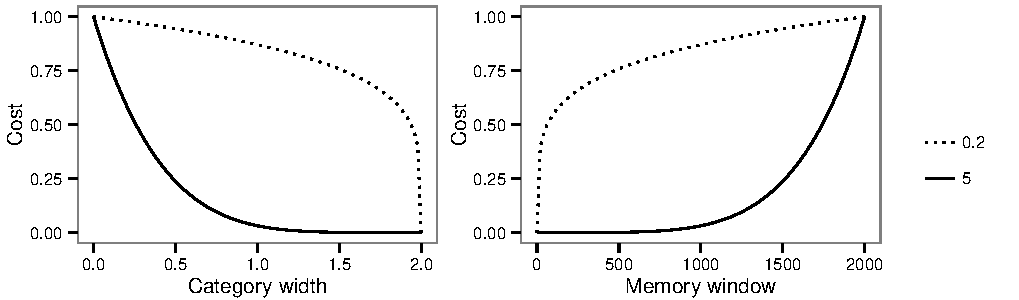
\includegraphics[width=.8\textwidth]{figures/cost_functions.pdf}
\caption{\sffamily\small\textbf{Cost functions.} Here we show how the cost functions for the cognitive parameters category width and memory window. In each panel, the solid line corresponds to $\alpha=5$ and the dotted line corresponds to $\alpha=0.2$. }
\label{cost_fx}
\end{figure}

\begin{figure}[ht]
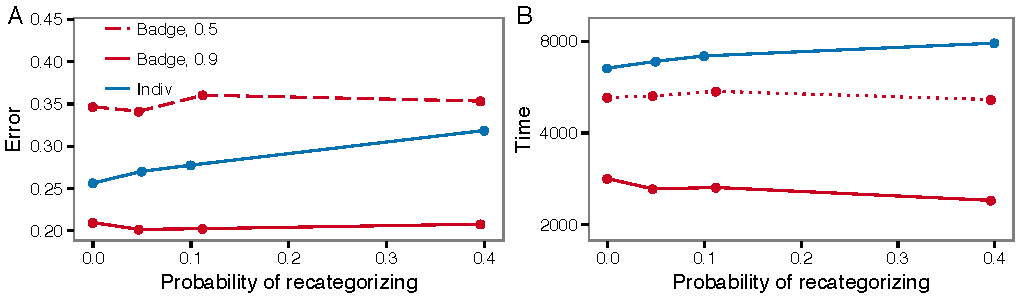
\includegraphics[width=6.85in]{figures/confusion_probs.pdf}
\caption{\sffamily\small\textbf{Increasing the probability of being confused increases error and learning time in the individual recognition system and decreases error and learning time in the badge system.} Error and learning time are minimized at an intermediate category width. In the left pane, we show average error $\bar{\epsilon}$ as a function of the probability of recategorizing, and in the right panel, we show average learning time $\bar{\tau}$ as a function of the probability of recategorizing. In each panel, blue lines show animals using individual recognition and red lines show animals using the badge system. The solid red lines correspond to groups in which the signal-quality correlation $\rho=0.9$ and the dotted lines correspond to groups in which the signal-quality correlation $\rho=0.5$. Parameters: $\delta = 0.5$, $\ell_\text{i}=0.2$, $N=50$, $p_\text{o}=0$, $\sigma_\text{b}=0.2$, $\sigma_\text{i}=0.01$, $\sigma_\text{q}=0.5$, $T=10000$, $w=1100$.}
\label{confusion_probs}
\end{figure}

\begin{figure}[ht]
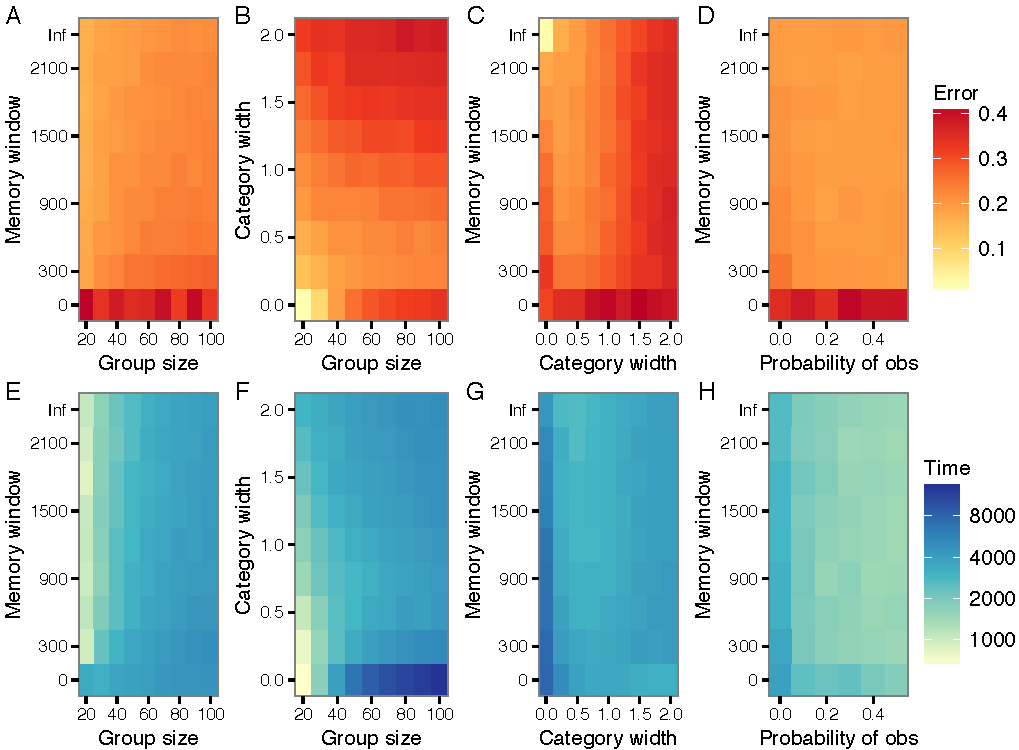
\includegraphics[width=.8\textwidth]{figures/parameter_interactions_badge.pdf}
\caption{\sffamily\small\textbf{Parameter interactions for animals using the badge system.}
In A, B, and C we show average error $\bar{\epsilon}$ for animals using the badge system as a function of two parameters. In D, E, and F we show average learning time $\bar{\tau}$ as a function of two parameters. Parameters: unless the parameter is being varied $\delta = 0.5$, $\ell_\text{i}=0.2$, $N=50$, $p_\text{o}=0$, $\rho=0.9$, $\sigma_\text{b}=0.2$, $\sigma_\text{i}=0.01$, $\sigma_\text{q}=0.5$, $T=10000$, $w=1100$.}
\label{interactions_badge}
\end{figure}

\begin{figure}[ht]
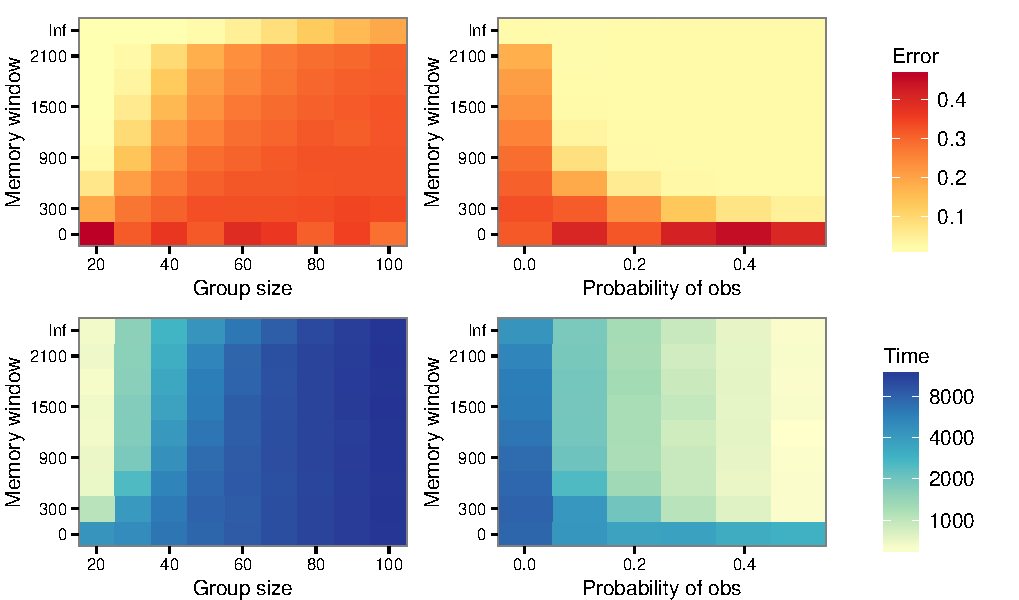
\includegraphics[width=.8\textwidth]{figures/parameter_interactions_indiv.pdf}
\caption{\sffamily\small\textbf{Parameter interactions for animals using individual recognition.}
In A, B, and C we show average error $\bar{\epsilon}$ for animals using individual recognition as a function of two parameters. In D, E, and F we show average learning time $\bar{\tau}$ as a function of two parameters. Parameters: unless the parameter is being varied $\delta = 0.5$, $\ell_\text{i}=0.2$, $N=50$, $p_\text{o}=0$, $\rho=0.9$, $\sigma_\text{b}=0.2$, $\sigma_\text{i}=0.01$, $\sigma_\text{q}=0.5$, $T=10000$, $w=1100$.}
\label{interactions_indiv}
\end{figure}

\begin{table}
\caption{\label{corr_examples} Examples of the correlation between a badge and a measure of fitness.}
\begin{tabular}{lllll}
Species & Badge & Measure of fitness & Reference
\\\hline paper wasp & percent black on face & body size (head width) & $r^2=0.36$  & \cite{Tibbetts:2004kx}
\\ & & & for wasps with $\geq 2$ black spots
\\ & ``badge brokenness" & dominance & $r^2=.105$ (multivariate) & \cite{Tibbetts:2004kx}
\\ \hline house sparrow & size of black bib & physical condition & $r=0.379$ & \cite{Veiga:1993fk}
\\ \hline swamp sparrow & size of rusty cap & parental investment & $r^2=0.33$ & \cite{Olsen:2010uq}
\\ & size of black forehead & aggression & $r^2=0.41$ & \cite{Olsen:2010uq}
\end{tabular}
\end{table}

\end{document}
